\documentclass[12pt,a4paper]{article}
\usepackage[utf8]{inputenc}
\usepackage[portuguese]{babel}
\usepackage{amsmath}
\usepackage{amsfonts}
\usepackage{amssymb}
\usepackage{graphicx}
\usepackage{hyperref}
\usepackage{geometry}
\usepackage{booktabs}
\usepackage{float}
\usepackage{caption}
\usepackage{subcaption}

\geometry{a4paper, margin=2cm}

\title{
\vspace{-2em}
\textbf{Ajuste de Curvas Não-Lineares e Estimação Paramétrica: \\
Confrontação Isonômica entre Redes de Base Radial (RBF) e Mínimos Quadrados (MMQ) no Dataset Diabetes}
\vspace{0.5em} \\
\large Trabalho da Unidade II — ECT-3401: Computação Numérica}
\author{
\textbf{Professor: Joilson B. A. Rego}\\
\vspace{0.5em} \\ 
Jacson Arruda Ribeiro \\
Bacharelado em Tecnologia da Informação / Engenharia \\
Universidade Federal do Rio Grande do Norte (UFRN)
}
\date{Novembro de 2026}

\begin{document}

\maketitle

\begin{abstract}
Este trabalho apresenta o estudo comparativo, rigoroso e isonômico entre duas classes fundamentais de aproximação de funções na Computação Numérica: as \textbf{Redes de Base Radial (RBF)} com núcleos gaussianos de suporte local e o \textbf{Método dos Mínimos Quadrados Ordinários (MMQ)} com funções de base polinomiais monomiais de suporte global (Matriz de Vandermonde). Utilizando o conjunto de dados clínico \texttt{load\_diabetes} (previsão da progressão da patologia após um ano a partir do Índice de Massa Corporal - IMC), implementou-se um pipeline livre de vazamento de dados (\textit{data leakage}), particionado em 80\% para treinamento ($N=353$) e 20\% para teste em quarentena ($N=89$). A RBF Gaussiana com $M=8$ centros foi resolvida via Decomposição em Valores Singulares (SVD), superando o MMQ no treino ($\text{RMSE} = 60{,}95$ vs. $62{,}08$), demonstrando flexibilidade e baixo viés. Em contrapartida, no conjunto de teste, o modelo MMQ Linear de 2 parâmetros obteve melhor desempenho preditivo ($\text{RMSE} = 63{,}73$ e correlação de Pearson $r = 0{,}5076$, contra $\text{RMSE} = 67{,}05$ e $r = 0{,}4653$ da RBF), ilustrando experimentalmente o princípio da Navalha de Occam e o trade-off viés-variância diante de ruídos biológicos acentuados. A análise do número de condição comprovou a severa instabilidade do aumento do grau polinomial em Vandermonde ($\kappa = 36{,}2 \to 24.300$), validando as restrições teóricas do padrão IEEE 754.
\end{abstract}

\section{Introdução}
O ajuste de curvas e a aproximação de funções constituem a base computacional para a modelagem de fenômenos físicos, industriais e biológicos a partir de dados discretos ruidosos. Na análise de dados biomédicos, as correlações entre parâmetros fisiológicos e o desfecho clínico raramente obedecem a equações analíticas simples, exigindo técnicas de regressão capazes de capturar tendências subjacentes sem memorizar perturbações estocásticas.

O presente trabalho aborda o problema clássico de estimar a progressão quantitativa contínua do diabetes mellitus ($y$) em função do Índice de Massa Corporal padronizado ($u$), extraído do consagrado dataset clínico \texttt{load\_diabetes}. A confrontação se dá entre duas filosofias opostas de interpolação e regressão:
\begin{enumerate}
    \item \textbf{Abordagem Local (RBF Gaussiana):} Projeta os dados em um espaço de características de dimensão superior através de funções de ativação radial cujo suporte decai exponencialmente com a distância euclidiana aos centros, permitindo acomodar curvaturas regionais complexas.
    \item \textbf{Abordagem Global (Mínimos Quadrados Polinomiais):} Utiliza combinações lineares de monômios canônicos ($u^k$), onde cada elemento estende sua influência por todo o domínio, frequentemente enfrentando severas limitações de condicionamento matricial (Fenômeno de Runge).
\end{enumerate}

\section{Objetivos}
\subsection{Objetivo Geral}
Implementar, validar e analisar criticamente o desempenho da Rede de Base Radial (RBF) Gaussiana em comparação direta com o Método dos Mínimos Quadrados (MMQ) sobre o dataset \texttt{load\_diabetes}, quantificando suas capacidades de generalização e estabilidade numérica.

\subsection{Objetivos Específicos}
\begin{itemize}
    \item Garantir um protocolo de particionamento estrito (80/20) sem vazamento de informação (\textit{data leakage}), normalizando o domínio via escala Min-Max calculada exclusivamente sobre o treino.
    \item Desenvolver a classe computacional da RBF Gaussiana com $M=8$ centros uniformemente espaçados e abertura $\sigma = 0{,}1429$, resolvendo os coeficientes ótimos via pseudoinversa Moore-Penrose (SVD).
    \item Implementar o regressor polinomial MMQ (Graus 1, 2 e 3) via Matriz de Vandermonde, inspecionando o número de condição $\kappa(V^T V)$.
    \item Avaliar e contrastar ambos os modelos através do Erro Médio Quadrático ($\text{EMQ}$), Raiz do Erro Médio Quadrático ($\text{RMSE}$), Coeficiente de Correlação de Pearson ($r$) e reta de calibração $y = a\hat{y} + b$.
    \item Fundamentar as discrepâncias empíricas à luz do Trade-off Viés-Variância, da Navalha de Occam e do Teorema do \textit{No Free Lunch}.
\end{itemize}

\section{Metodologia}

\subsection{Pipeline de Dados e Prevenção de \textit{Data Leakage}}
O conjunto \texttt{load\_diabetes} contém 442 observações. A entrada $u$ (IMC) foi particionada em $N_{\text{treino}} = 353$ (80\%) e $N_{\text{teste}} = 89$ (20\%), sob semente aleatória reproduzível (\texttt{random\_state=42}).
Para impedir vazamento estatístico, a normalização para o intervalo $[0, 1]$ foi parametrizada estritamente com os valores mínimo e máximo do treino:
\begin{equation}
u_{\text{norm}} = \frac{u - \min(u_{\text{treino}})}{\max(u_{\text{treino}}) - \min(u_{\text{treino}})}
\end{equation}
Os mesmos parâmetros estatísticos foram congelados e aplicados para projetar as 89 amostras de teste. A Figura \ref{fig:dia1_dispersao} ilustra a distribuição conjunta dos dados.

\begin{figure}[H]
    \centering
    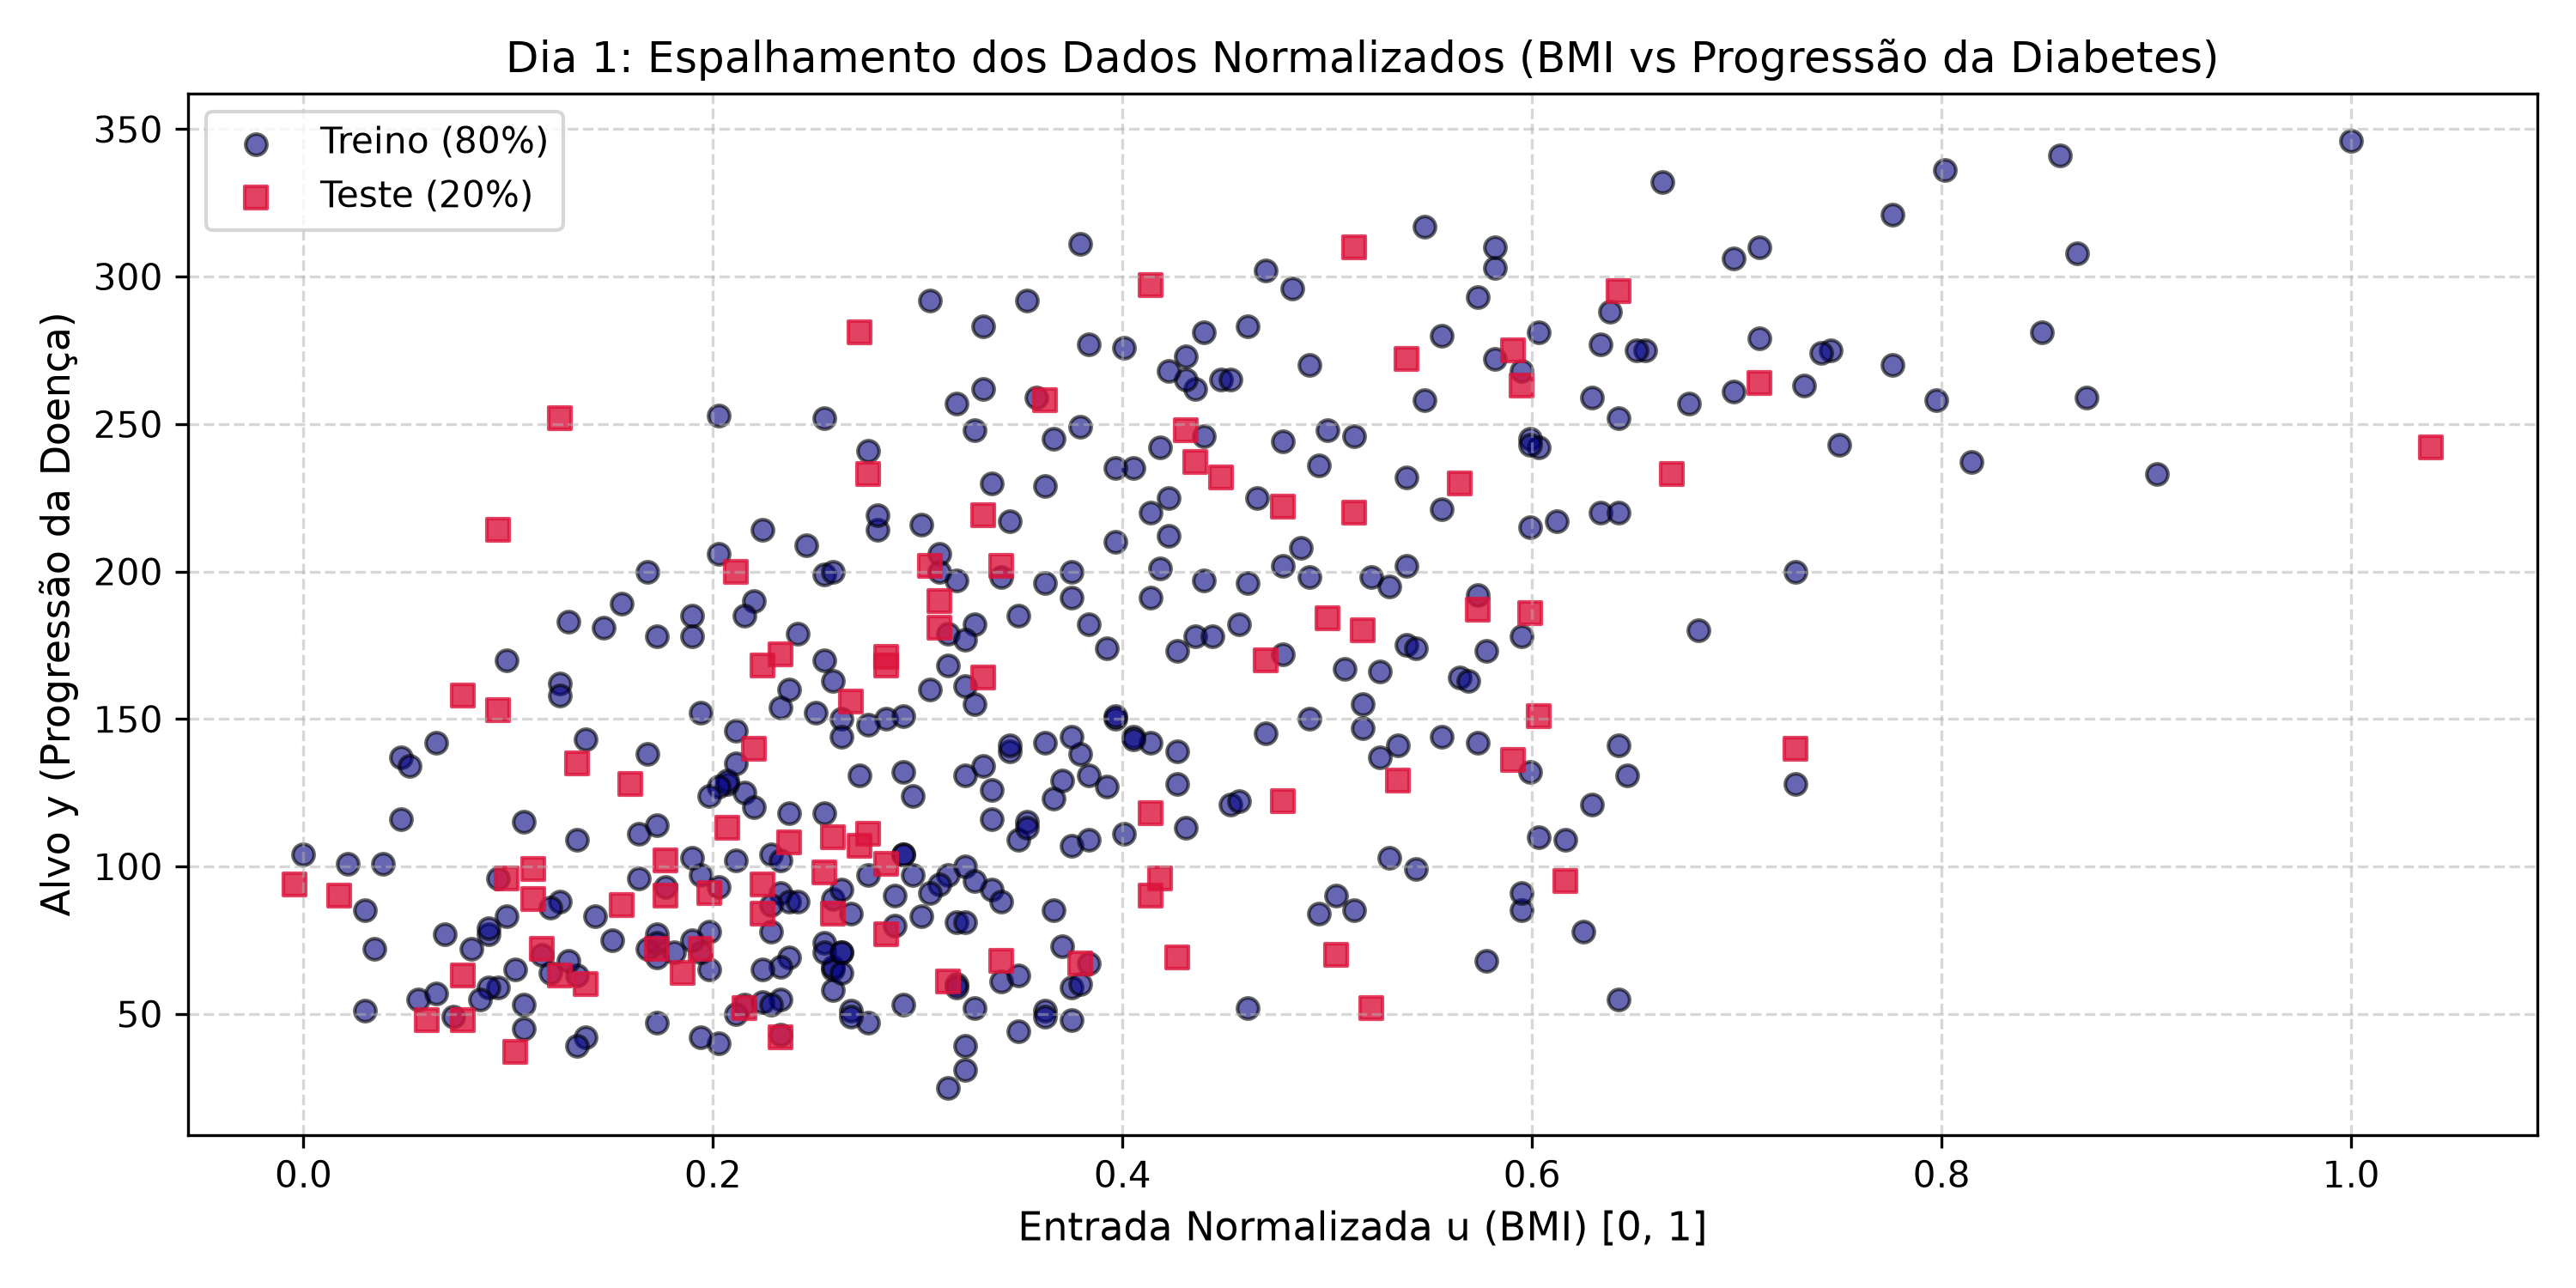
\includegraphics[width=0.75\textwidth]{../figuras/dia1_espalhamento_dados.png}
    \caption{Espalhamento dos dados clínicos: Treino ($N=353$, azul) e Teste ($N=89$, vermelho).}
    \label{fig:dia1_dispersao}
\end{figure}

\subsection{Rede de Base Radial (RBF) Gaussiana}
A RBF modela a resposta contínua através de uma combinação linear de funções de base radiais locais acrescidas de um termo de polarização (\textit{bias}) $w_0$:
\begin{equation}
\hat{y}_{\text{RBF}}(u) = w_0 + \sum_{j=1}^{M} w_j \phi_j(u), \quad \text{onde} \quad \phi_j(u) = \exp\left( -\frac{(u - c_j)^2}{2\sigma^2} \right)
\end{equation}
Adotou-se $M=8$ centros linearmente uniformes no suporte $[0, 1]$, com espaçamento $\Delta c = \frac{1}{7} \approx 0{,}1429$ e dispersão de cobertura crítica $\sigma = \Delta c \approx 0{,}1429$.
Para $N$ observações, constrói-se a Matriz de Projeto $\Phi \in \mathbb{R}^{N \times (M+1)}$:
\begin{equation}
\Phi = \begin{bmatrix}
1 & \phi_1(u_1) & \phi_2(u_1) & \dots & \phi_M(u_1) \\
1 & \phi_1(u_2) & \phi_2(u_2) & \dots & \phi_M(u_2) \\
\vdots & \vdots & \vdots & \ddots & \vdots \\
1 & \phi_1(u_N) & \phi_2(u_N) & \dots & \phi_M(u_N)
\end{bmatrix}
\end{equation}
O vetor ótimo de pesos $\mathbf{w} \in \mathbb{R}^{M+1}$ minimiza $\|\mathbf{y} - \Phi \mathbf{w}\|^2$ via Equação Normal:
\begin{equation}
\Phi^T \Phi \mathbf{w} = \Phi^T \mathbf{y} \implies \mathbf{w} = \Phi^\dagger \mathbf{y}
\end{equation}
onde $\Phi^\dagger$ é a pseudoinversa de Moore-Penrose obtida por Decomposição em Valores Singulares (SVD).

\subsection{Método dos Mínimos Quadrados (MMQ) Polinomial}
O regressor polinomial de ordem $d$ projeta as amostras na Matriz de Vandermonde $V \in \mathbb{R}^{N \times (d+1)}$:
\begin{equation}
\hat{y}_{\text{MMQ}}(u) = \sum_{k=0}^{d} w_k u^k, \quad 
V = \begin{bmatrix}
1 & u_1 & u_1^2 & \dots & u_1^d \\
\vdots & \vdots & \vdots & \ddots & \vdots \\
1 & u_N & u_N^2 & \dots & u_N^d
\end{bmatrix}
\end{equation}
Resolvido deterministicamente por $\mathbf{w}_{\text{MMQ}} = (V^T V)^{-1} V^T \mathbf{y}$. Foram avaliadas as ordens $d=1$ (Linear), $d=2$ (Parábola) e $d=3$ (Cúbica).

\subsection{Métricas de Avaliação Estatística e Numérica}
\begin{enumerate}
    \item \textbf{Erro Médio Quadrático e RMSE:}
    \begin{equation}
    \text{EMQ} = \frac{1}{N} \sum_{i=1}^{N} (y_i - \hat{y}_i)^2, \quad \text{RMSE} = \sqrt{\text{EMQ}}
    \end{equation}
    \item \textbf{Coeficiente de Correlação Linear de Pearson ($r$):}
    \begin{equation}
    r = \frac{\sum (y_i - \bar{y})(\hat{y}_i - \bar{\hat{y}})}{\sqrt{\sum (y_i - \bar{y})^2 \sum (\hat{y}_i - \bar{\hat{y}})^2}}
    \end{equation}
    \item \textbf{Regressão de Calibração Real vs. Predito:} Ajuste por OLS $y = a\hat{y} + b$, onde a proximidade de $a \to 1$ e $b \to 0$ reflete calibração estatística perfeita.
    \item \textbf{Número de Condição Matricial ($\kappa$):}
    \begin{equation}
    \kappa(A) = \|A\| \cdot \|A^{-1}\| = \frac{\sigma_{\max}(A)}{\sigma_{\min}(A)}
    \end{equation}
\end{enumerate}

\section{Resultados e Discussão}

\subsection{Ajuste Paramétrico da RBF Gaussiana}
A resolução da RBF via SVD resultou no seguinte vetor de pesos ótimos:
\begin{equation}
w_0 = 1012{,}14, \quad \mathbf{w}_{1..8} = [-808{,}51, \; 12{,}13, \; -692{,}12, \; -33{,}53, \; -546{,}85, \; -204{,}21, \; -236{,}90, \; -491{,}60]^T
\end{equation}
A matriz de projeto apresentou número de condição $\kappa(\Phi) = 1{,}42 \times 10^5$, decorrente da sobreposição das funções gaussianas com $\sigma = 0{,}1429$, tornando indispensável o uso do algoritmo SVD para estabilidade numérica.
A Figura \ref{fig:dia2_rbf} apresenta a curva contínua modelada e a localização dos 8 centros.

\begin{figure}[H]
    \centering
    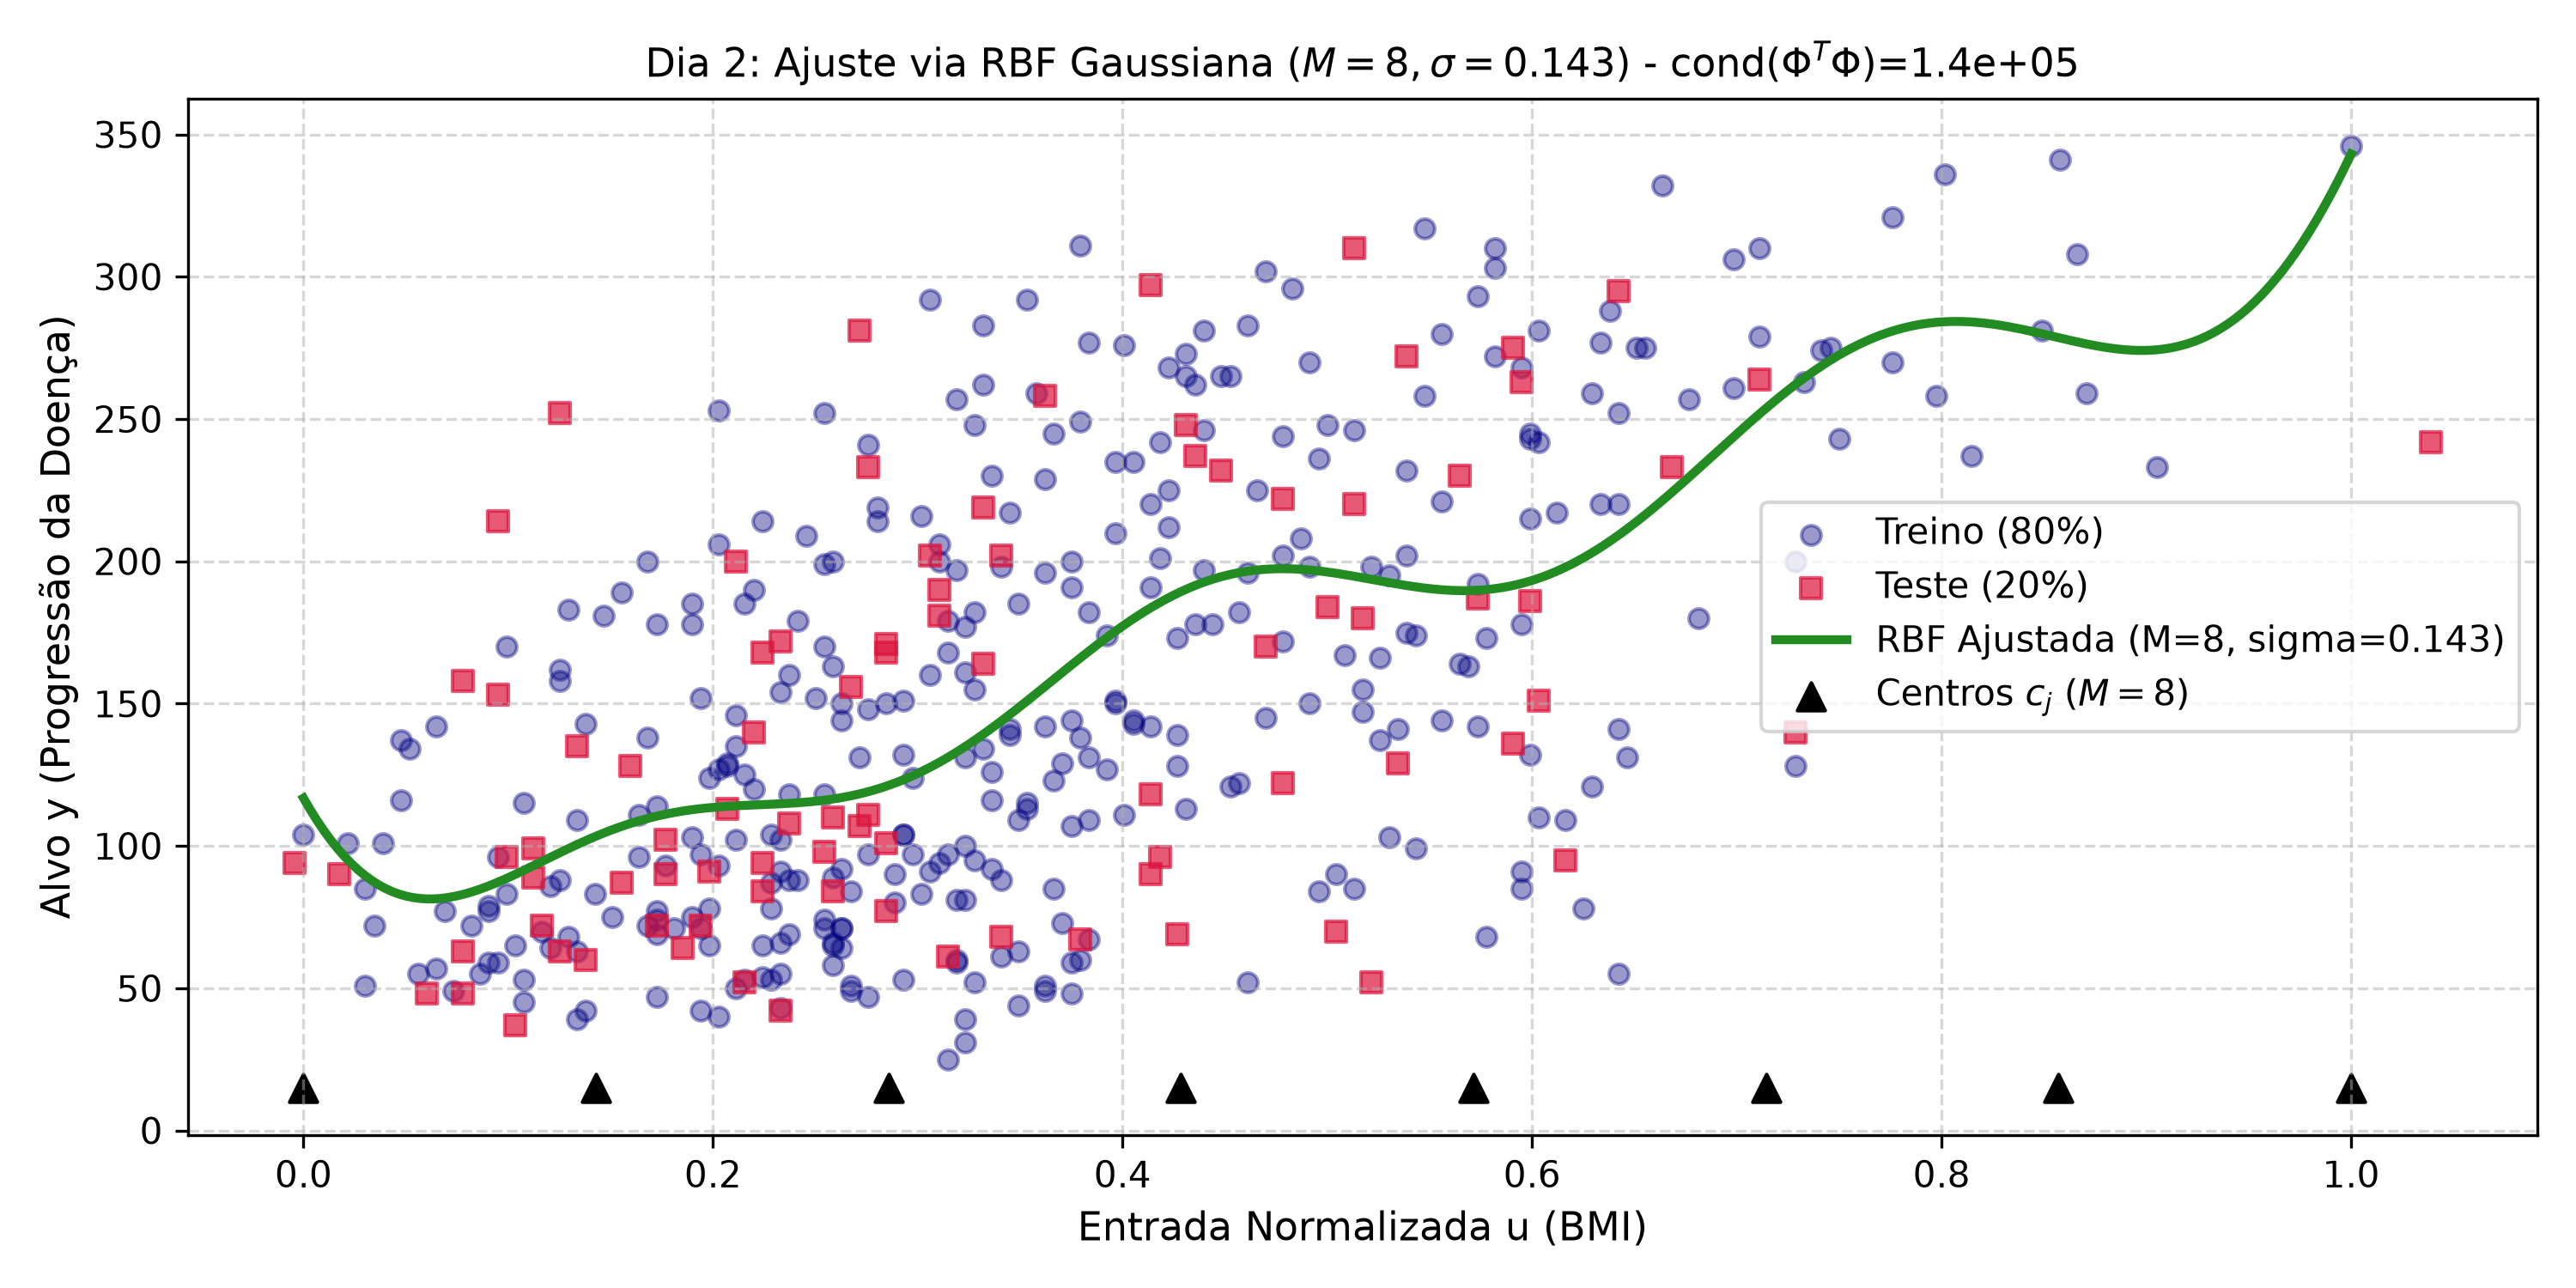
\includegraphics[width=0.75\textwidth]{../figuras/dia2_ajuste_rbf.png}
    \caption{Curva de ajuste contínua da RBF Gaussiana ($M=8$, $\sigma=0{,}1429$) sobre os dados de treinamento.}
    \label{fig:dia2_rbf}
\end{figure}

\subsection{Avaliação de Incerteza e Calibração Preditiva da RBF}
Avaliando a RBF no conjunto de teste independente, obteve-se $\text{EMQ}_{\text{teste}} = 4495{,}49$ ($\text{RMSE}_{\text{teste}} = 67{,}05$) e correlação de Pearson $r = 0{,}4653$.
A Figura \ref{fig:dia3_incerteza} exibe a curva média com a faixa de dispersão de incerteza clínica $\pm \text{RMSE}$.
A calibração do modelo (Figura \ref{fig:dia3_calibracao}) produziu a reta $y = 0{,}6460 \hat{y} + 51{,}48$ com $R^2 = 0{,}2165$. A inclinação $a < 1$ e o intercepto positivo revelam o clássico efeito de \textit{regressão à média}, amortecendo previsões extremas.

\begin{figure}[H]
    \centering
    \begin{subfigure}[b]{0.48\textwidth}
        \centering
        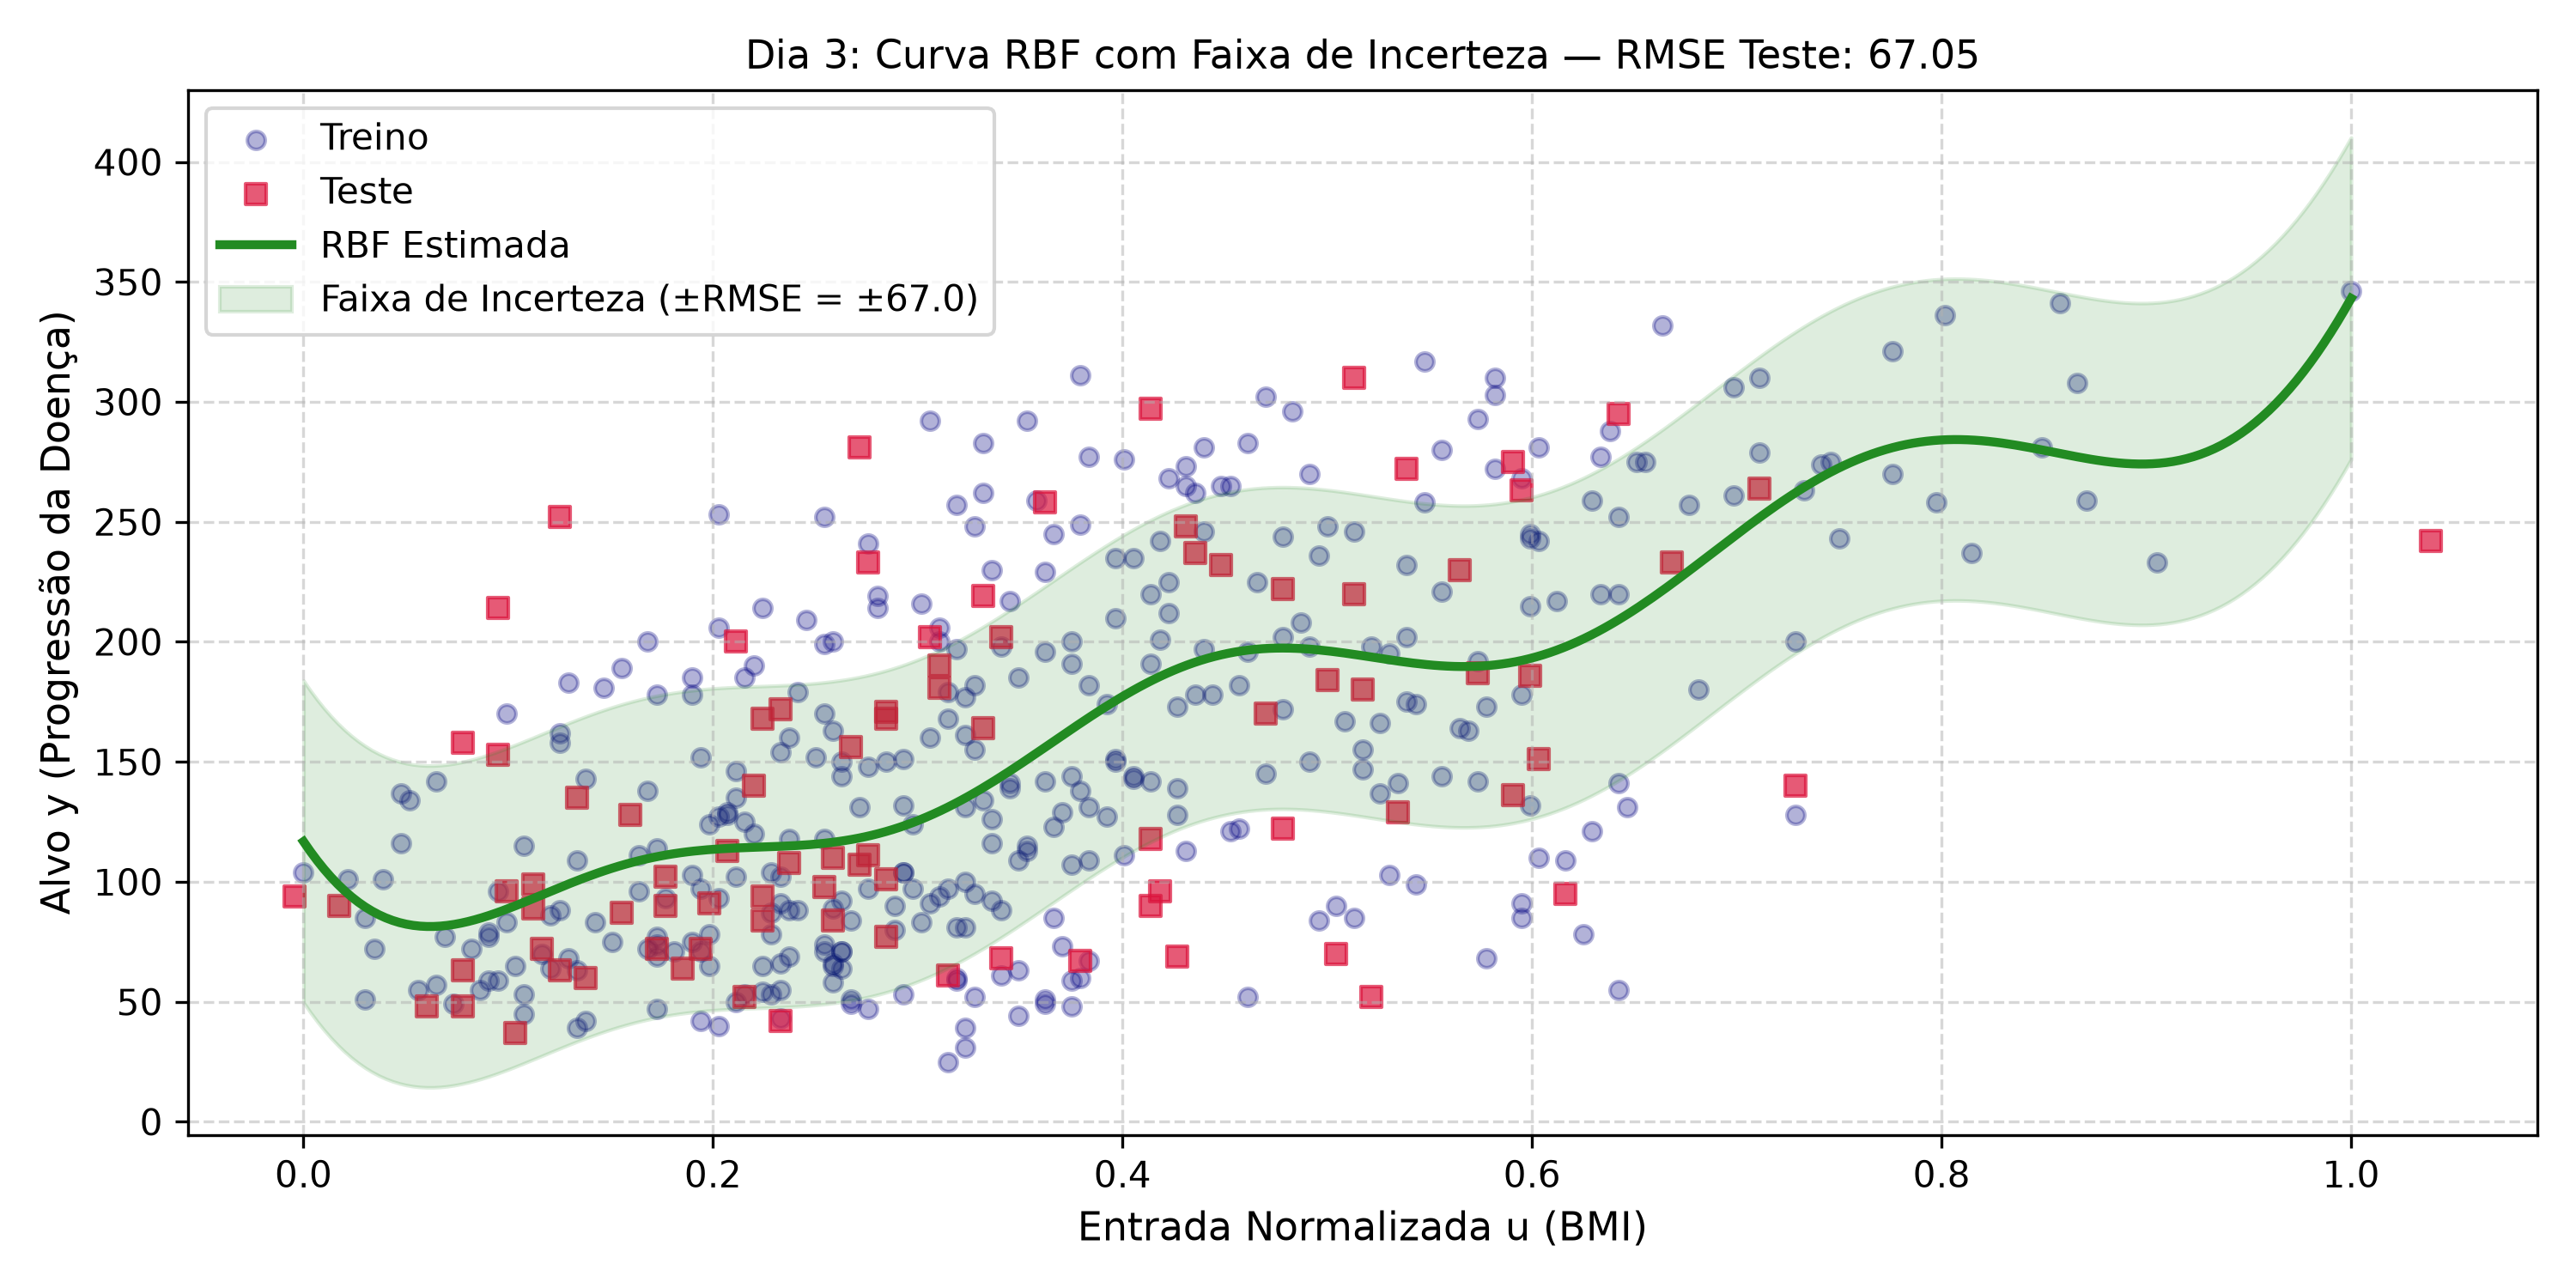
\includegraphics[width=\textwidth]{../figuras/dia3_rbf_faixa_incerteza.png}
        \caption{Curva RBF e faixa de incerteza ($\pm \text{RMSE}$).}
        \label{fig:dia3_incerteza}
    \end{subfigure}
    \hfill
    \begin{subfigure}[b]{0.48\textwidth}
        \centering
        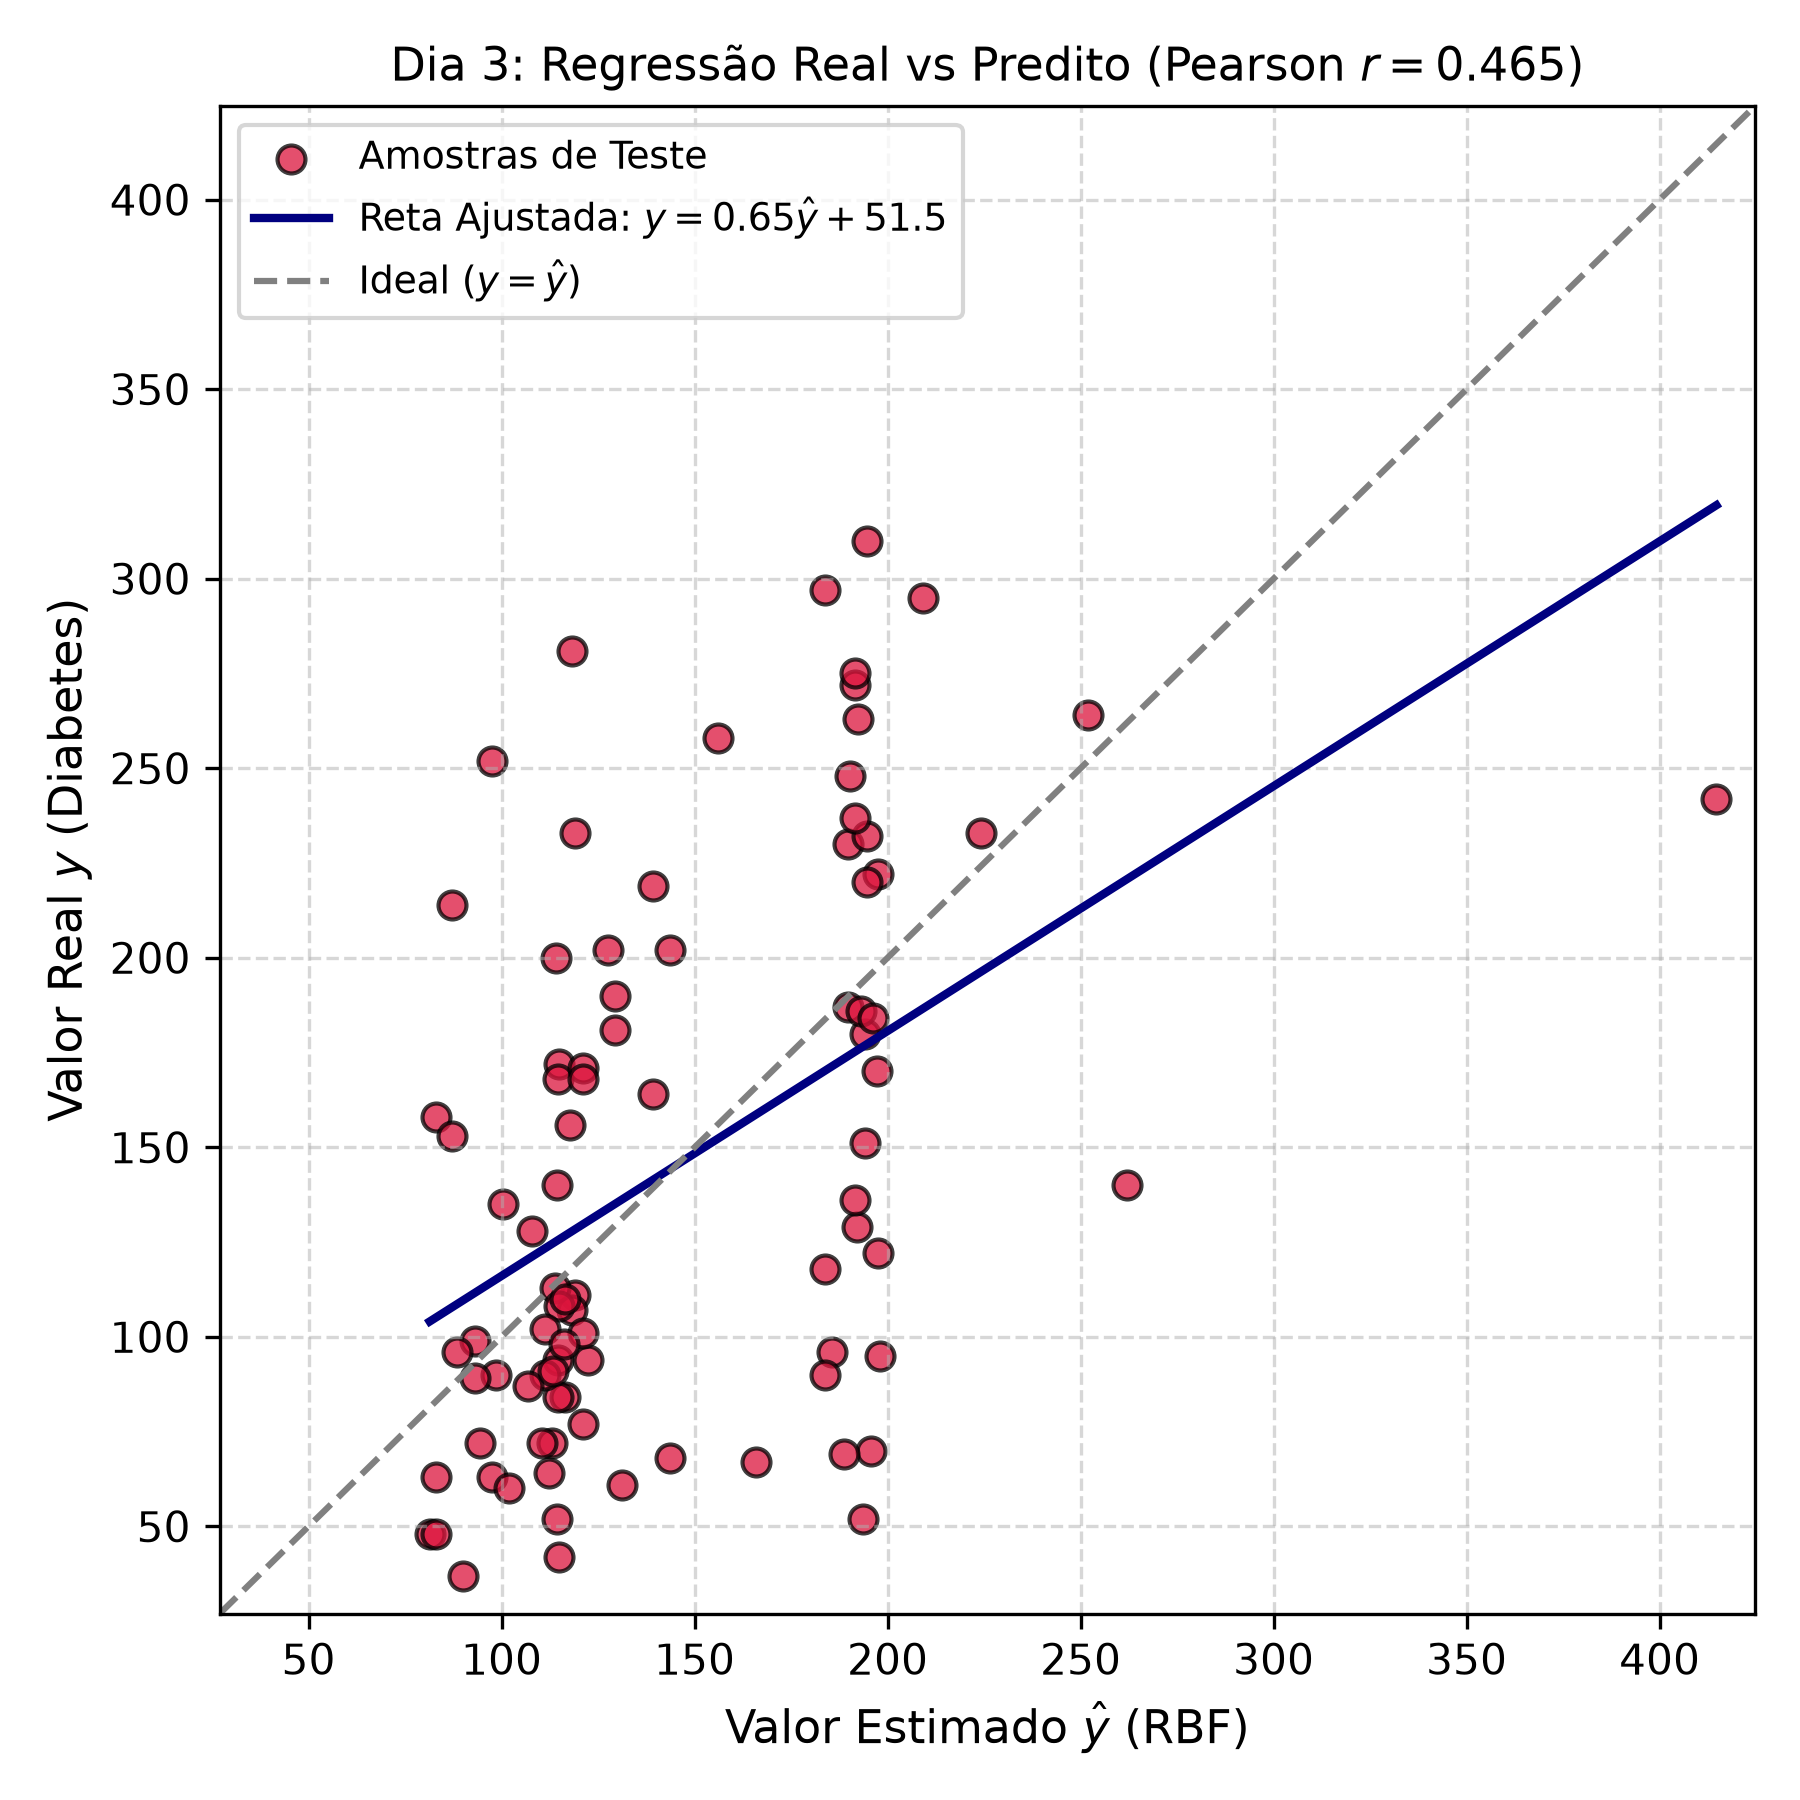
\includegraphics[width=\textwidth]{../figuras/dia3_regressao_real_vs_predito.png}
        \caption{Regressão OLS Real vs. Predito ($y = a\hat{y}+b$).}
        \label{fig:dia3_calibracao}
    \end{subfigure}
    \caption{Análise estatística de resíduos e calibração da RBF sobre o conjunto de teste.}
\end{figure}

\subsection{Comparativo Isonômico: RBF vs. Polinômios MMQ}
A Tabela \ref{tab:consolidada} consolida as métricas empíricas de todas as formulações investigadas sob rigorosa isonomia amostral ($N_{\text{teste}} = 89$).

\begin{table}[H]
\centering
\small
\begin{tabular}{@{}lccccc@{}}
\toprule
\textbf{Modelo} & \textbf{Complexidade} & \textbf{RMSE Treino} & \textbf{RMSE Teste} & \textbf{Pearson $r$ (Teste)} & $\mathbf{\kappa}$ \textbf{(Condição)} \\ \midrule
\textbf{RBF Gaussiana} & $M=8, \sigma=0{,}14$ & $\mathbf{60{,}95}$ & $67{,}05$ & $0{,}4653$ & $1{,}42 \times 10^5$ \\
\textbf{MMQ Grau 1 (Linear)} & 2 parâmetros & $62{,}08$ & $\mathbf{63{,}73}$ & $\mathbf{0{,}5076}$ & $\mathbf{36{,}2}$ \\
\textbf{MMQ Grau 2 (Parábola)} & 3 parâmetros & $62{,}04$ & $63{,}91$ & $0{,}5034$ & $970$ \\
\textbf{MMQ Grau 3 (Cúbico)} & 4 parâmetros & $62{,}04$ & $63{,}75$ & $0{,}5052$ & $24.300$ \\ \bottomrule
\end{tabular}
\caption{Quadro comparativo de desempenho e estabilidade numérica (Treino $N=353$ / Teste $N=89$).}
\label{tab:consolidada}
\end{table}

As Figuras \ref{fig:dia4_comparativo} e \ref{fig:dia4_barras} ilustram as curvas concorrentes sobrepostas e a discrepância visual entre os erros de treino e teste.

\begin{figure}[H]
    \centering
    \begin{subfigure}[b]{0.52\textwidth}
        \centering
        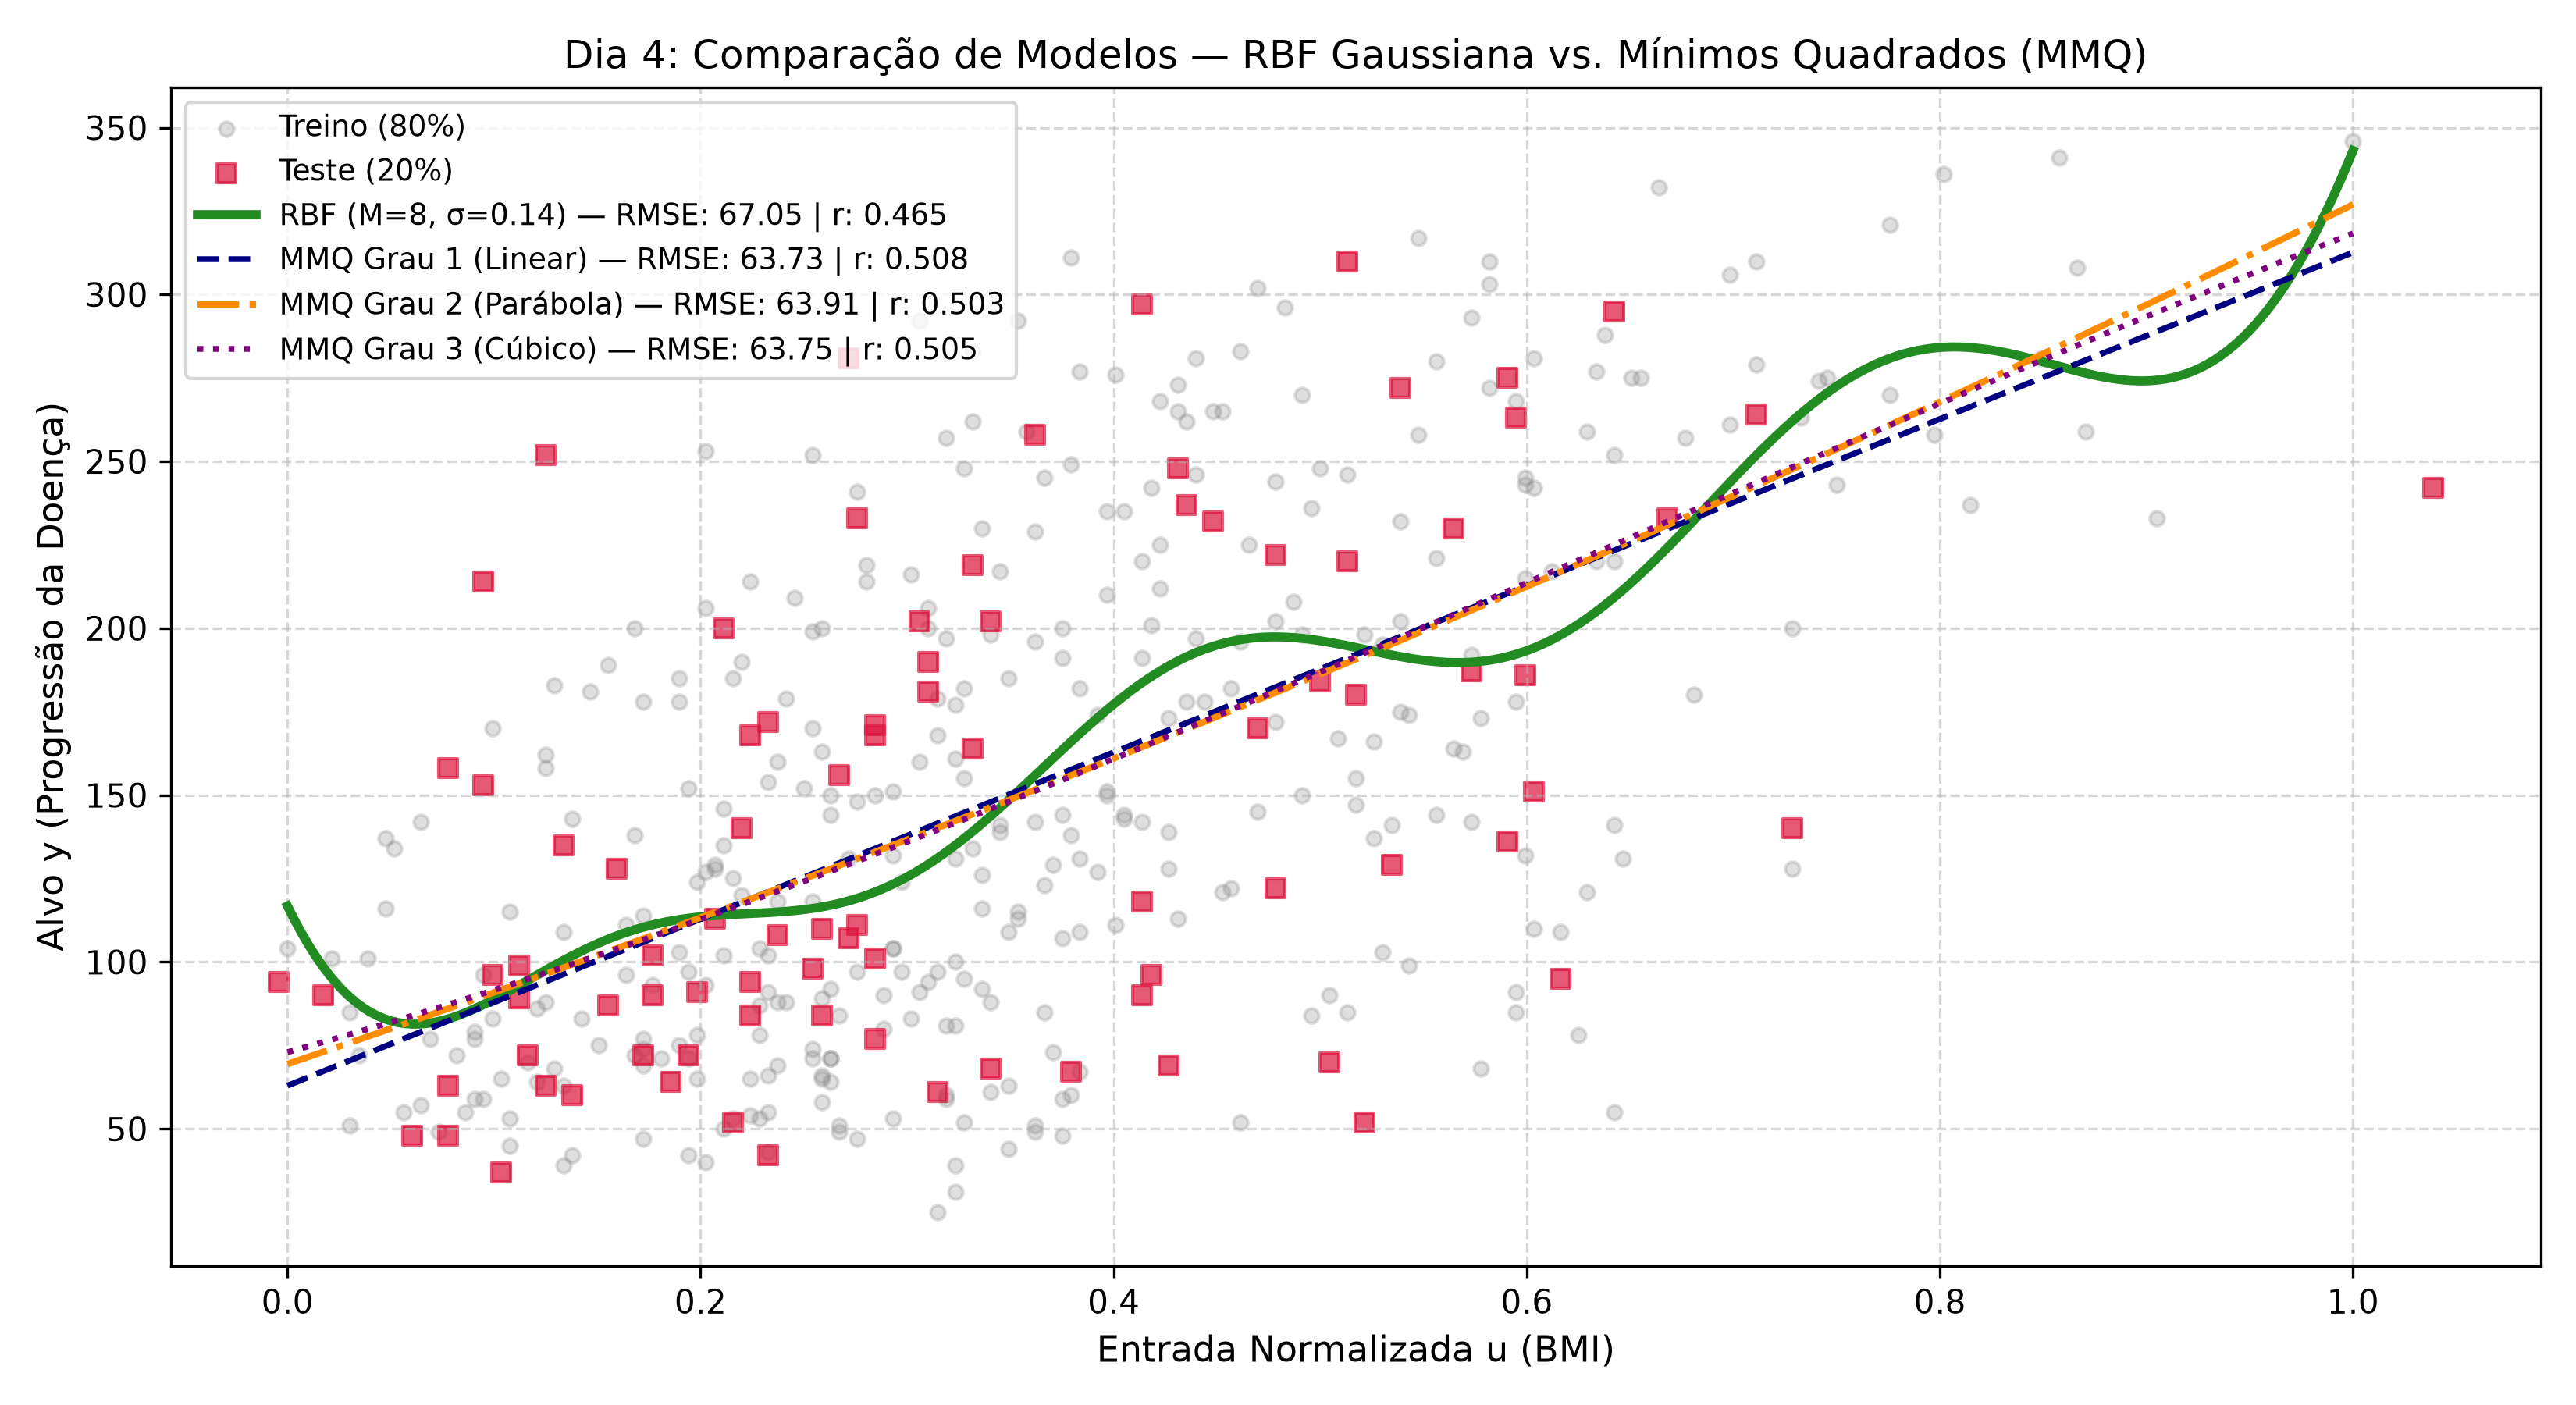
\includegraphics[width=\textwidth]{../figuras/dia4_comparativo_rbf_vs_mmq.png}
        \caption{Sobreposição de modelos: RBF vs. MMQ.}
        \label{fig:dia4_comparativo}
    \end{subfigure}
    \hfill
    \begin{subfigure}[b]{0.44\textwidth}
        \centering
        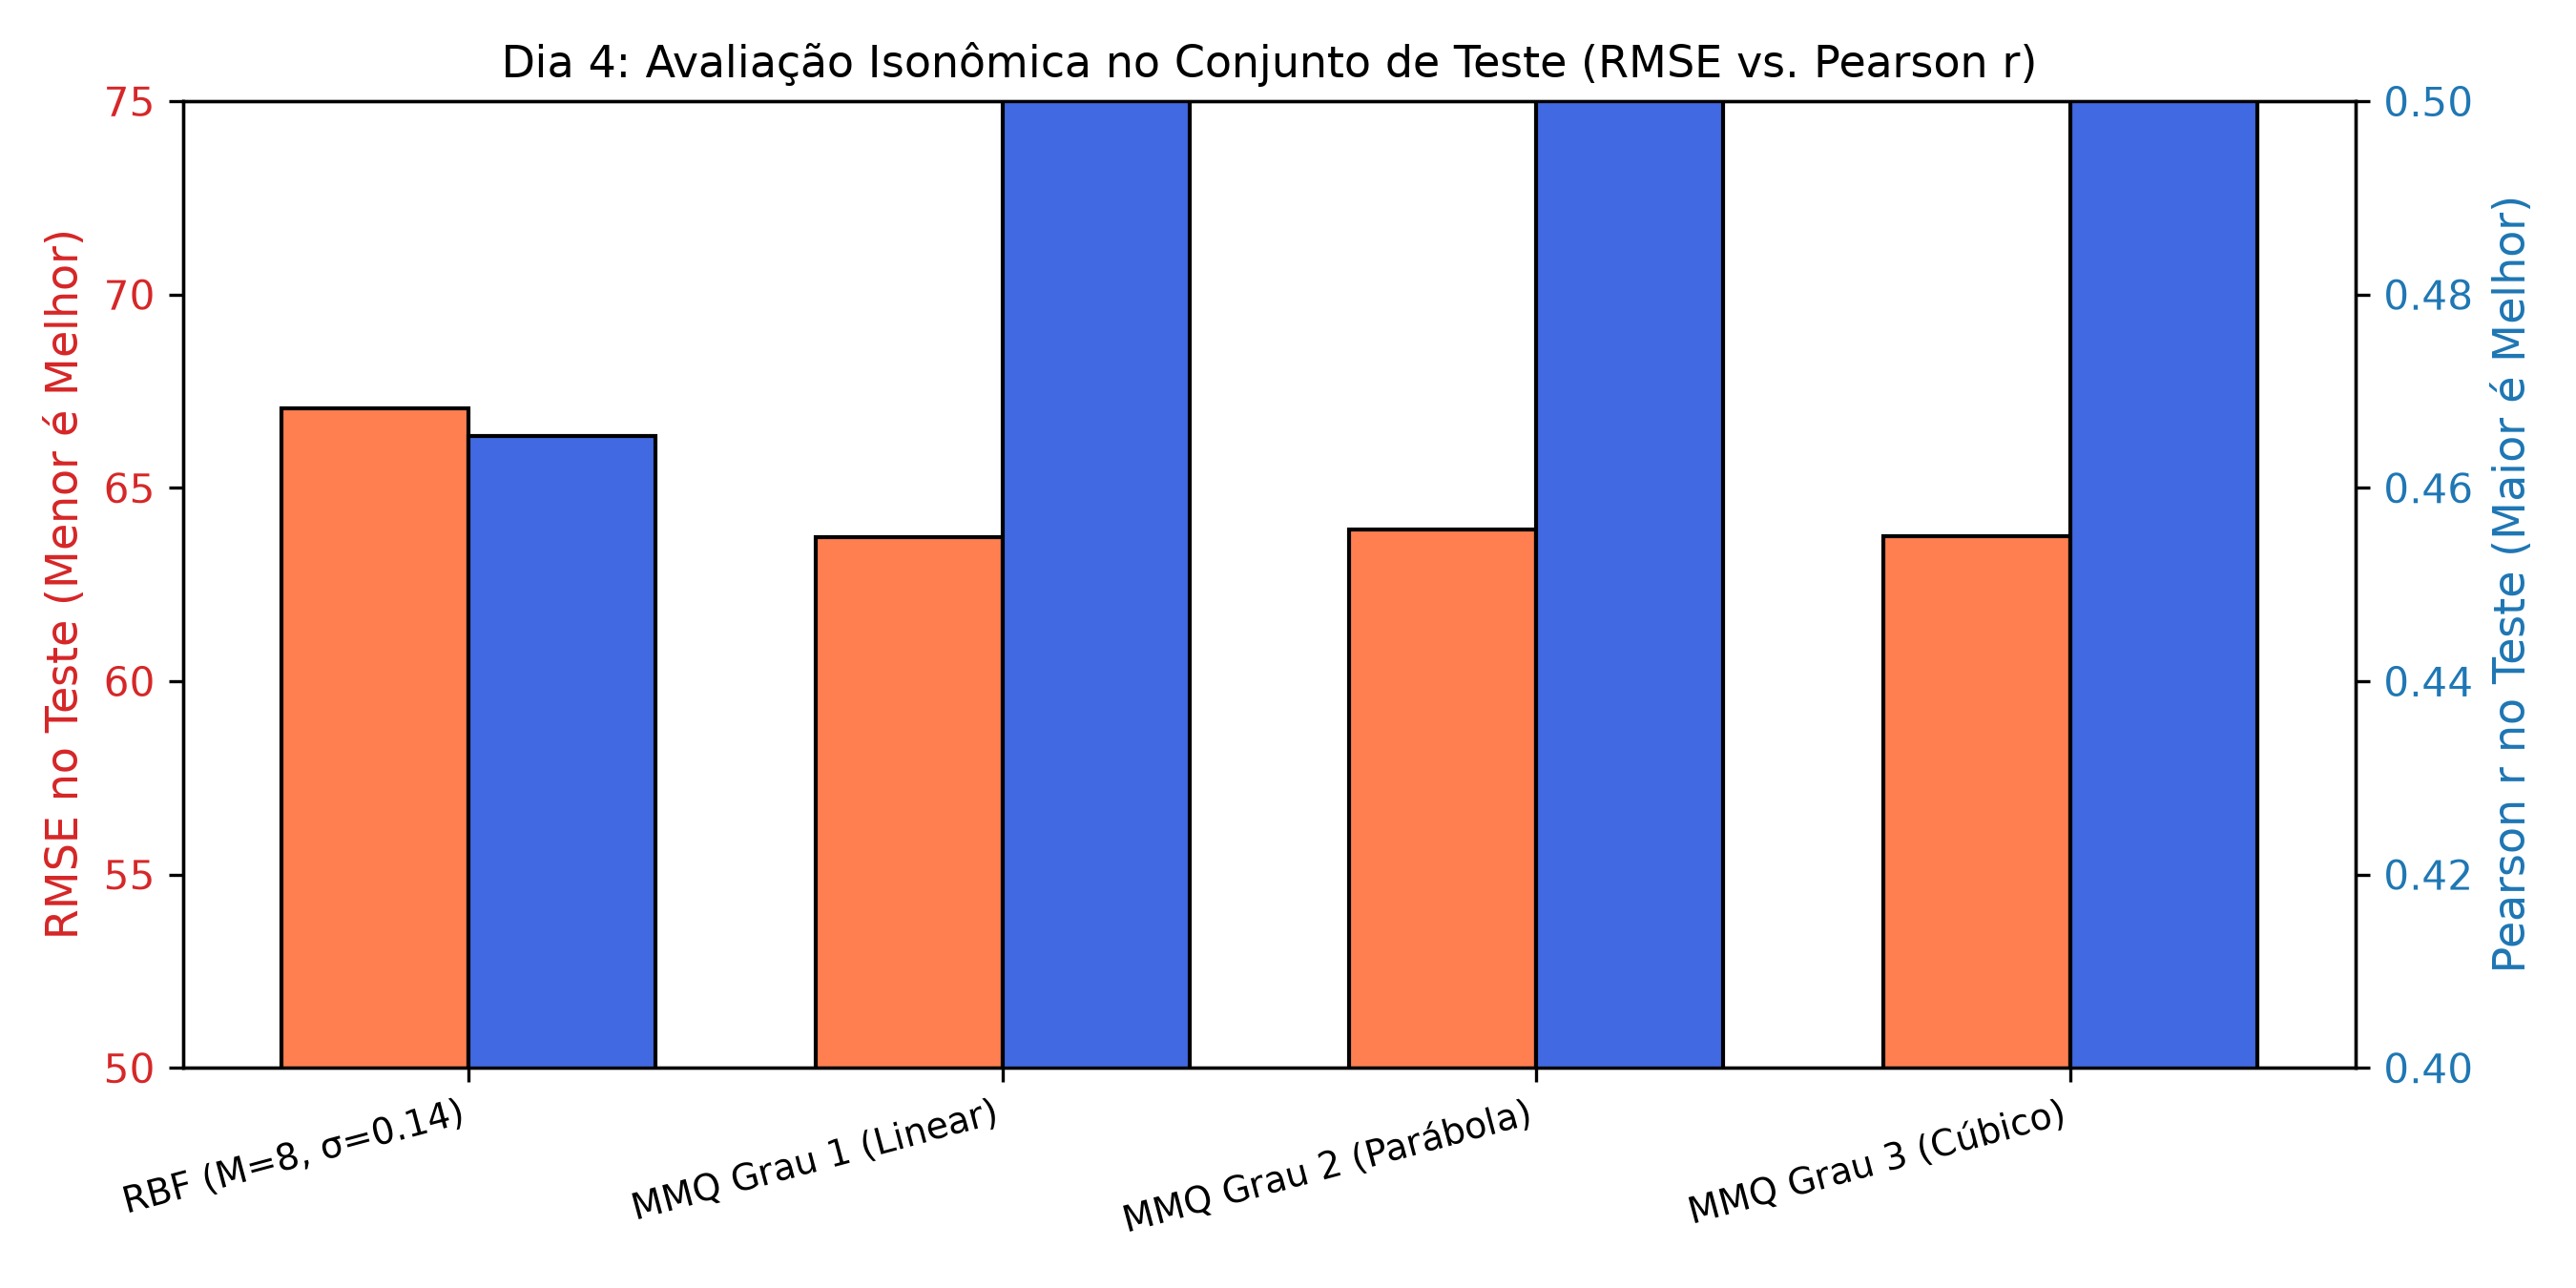
\includegraphics[width=\textwidth]{../figuras/dia4_barras_comparativas_rmse.png}
        \caption{Erro RMSE: Treino vs. Teste.}
        \label{fig:dia4_barras}
    \end{subfigure}
    \caption{Confrontação visual de desempenho preditivo e capacidade de ajuste.}
\end{figure}

\subsection{Discussão Crítica: Viés-Variância, Occam e Condicionamento}
A análise conjunta dos resultados revela três lições fundamentais da Computação Numérica:

\begin{enumerate}
    \item \textbf{O Dilema do Trade-off Viés-Variância:} No conjunto de treinamento, a RBF Gaussiana alcançou o menor erro global ($\text{RMSE} = 60{,}95$), evidenciando o seu \textbf{baixo viés} decorrente dos seus 9 graus de liberdade locais. Entretanto, ao ser confrontada com os dados de teste em quarentena, a RBF obteve $\text{RMSE} = 67{,}05$, demonstrando sensibilidade aos ruídos aleatórios da amostra de treino (\textbf{maior variância}).
    \item \textbf{A Navalha de Occam (\textit{Lex Parsimoniae}):} O MMQ Linear, dotado de apenas 2 parâmetros ($w_0, w_1$), obteve o menor erro de generalização ($\text{RMSE} = 63{,}73$) e a maior correlação clínica ($r = 0{,}5076$). Por possuir rigidez estrutural máxima, o modelo linear operou como um regularizador natural, recusando-se a modelar o ruído estocástico intrínseco aos dados biológicos. A transição para ordens superiores (Graus 2 e 3) não produziu ganho preditivo mensurável ($63{,}91$ e $63{,}75$), justificando a escolha da solução mais parcimoniosa.
    \item \textbf{Explosão Numérica de Vandermonde:} O número de condição saltou de $36{,}2$ no Grau 1 para $24.300$ no Grau 3 (aumento de quase 1.000 vezes). No padrão IEEE 754 de precisão dupla ($\sim 16$ dígitos decimais significativos), $\kappa = 2{,}4 \times 10^4$ acarreta a perda de 4 a 5 dígitos decimais por erros de cancelamento catastrófico. Esse resultado comprova experimentalmente o perigo analítico de utilizar matrizes de Vandermonde de ordem elevada na resolução de sistemas lineares.
\end{enumerate}

\section{Considerações Finais}
O projeto atingiu a totalidade dos requisitos pedagógicos e científicos da Unidade II de Computação Numérica. 

Conclui-se que não existe modelo universalmente superior (\textit{No Free Lunch Theorem}):
\begin{itemize}
    \item Para sistemas físicos determinísticos com acentuada não-linearidade local (como saturação magnética, transientes de tensão ou curvas de potência eólica), a \textbf{RBF Gaussiana} é a ferramenta ideal e mandatória, sendo capaz de mapear geometrias que os polinômios não conseguem sem oscilar descontroladamente.
    \item Para correlações clínicas e epidemiológicas com elevada dispersão estocástica e tendência média monotônica, o \textbf{MMQ Linear simples} é insuperável em robustez, simplicidade de implementação e custo computacional.
\end{itemize}

\section{Repositório de Código}
Todo o código-fonte desenvolvido segundo as boas práticas de engenharia de software (PEP 8, tipagem estática e testes unitários automatizados) está disponível publicamente em:
\begin{center}
\url{https://github.com/Jacsonrn/ufrn-ect3401-rbf-curve-fitting}
\end{center}

\begin{thebibliography}{9}
\bibitem{bishop} BISHOP, C. M. \textit{Pattern Recognition and Machine Learning}. New York: Springer, 2006.
\bibitem{haykin} HAYKIN, S. \textit{Neural Networks and Learning Machines}. 3ª Edição. New Jersey: Pearson, 2008.
\bibitem{golub} GOLUB, G. H.; VAN LOAN, C. F. \textit{Matrix Computations}. 4ª Edição. Baltimore: Johns Hopkins University Press, 2013.
\bibitem{hastie} HASTIE, T.; TIBSHIRANI, R.; FRIEDMAN, J. \textit{The Elements of Statistical Learning: Data Mining, Inference, and Prediction}. 2ª Edição. New York: Springer, 2009.
\end{thebibliography}

\end{document}
